\documentclass[14pt]{beamer}
%%%%%%%%%%%%%%%%%%%%%%%%%%%%%%%%%%%%%%%%%%%%%%%%%%%%%%%%%%%%%
% Meta informations:
\newcommand{\trauthor}{Jan Fabian Schmid}
\newcommand{\trtype}{Seminar} %{Proseminar} {Seminar} %{Workshop}
\newcommand{\trcourse}{Bio-inspired Artificial Intelligence}
\newcommand{\trtitle}{Effects of encoding on the general learning ability of ANNs}
\newcommand{\trmatrikelnummer}{6440383}
\newcommand{\tremail}{2schmid@informatik.uni-hamburg.de}
\newcommand{\trinstitute}{Dept. Informatik -- Knowledge Technology, WTM}
\newcommand{\trwebsiteordate}{{http://www.informatik.uni-hamburg.de/WTM/}}

%%%%%%%%%%%%%%%%%%%%%%%%%%%%%%%%%%%%%%%%%%%%%%%%%%%%%%%%%%%%%
% Languages:

% Falls die Ausarbeitung in Deutsch erfolgt:
% \usepackage[german]{babel}
% \usepackage[T1]{fontenc}
% \usepackage[latin1]{inputenc}
% \usepackage[latin9]{inputenc}	 				
% \selectlanguage{german}

% If the thesis is written in English:
\usepackage[english]{babel} 						
\selectlanguage{english}

%%%%%%%%%%%%%%%%%%%%%%%%%%%%%%%%%%%%%%%%%%%%%%%%%%%%%%%%%%%%%
% Bind packages:
\usepackage{beamerthemesplit}
\usetheme{Boadilla}
%\usetheme{Copenhagen}
%\usetheme{Darmstadt}
%\usetheme{Frankfurt}
%\usetheme{Ilmenau}
%\usetheme{JuanLesPins}
%\usetheme{Madrid}
%\usetheme{Warsaw }
%\usecolortheme{dolphin}
%\setbeamertemplate{sections/subsections in toc}[sections numbered]
%\beamertemplatenavigationsymbolsempty
%\setbeamertemplate{headline}[default] 	% deaktiviert die Kopfzeile
\setbeamertemplate{navigation symbols}{}% deaktiviert Navigationssymbole
%\useinnertheme{rounded}

\usepackage{acronym}                    % Acronyms
\usepackage{algorithmic}								% Algorithms and Pseudocode
\usepackage{algorithm}									% Algorithms and Pseudocode
\usepackage{amsfonts}                   % AMS Math Packet (Fonts)
\usepackage{amsmath}                    % AMS Math Packet
\usepackage{amssymb}                    % Additional mathematical symbols
\usepackage{amsthm}
\usepackage{color}                      % Enables defining of colors via \definecolor
\usepackage{fancybox}                   % Gleichungen einrahmen
\usepackage{fancyhdr}										% Paket zur schickeren der Gestaltung der 
\usepackage{graphicx}                   % Inclusion of graphics
%\usepackage{latexsym}                  % Special symbols
\usepackage{longtable}									% Allow tables over several parges
\usepackage{listings}                   % Nicer source code listings
\usepackage{lmodern}
\usepackage{multicol}										% Content of a table over several columns
\usepackage{multirow}										% Content of a table over several rows
\usepackage{rotating}										% Alows to rotate text and objects
\usepackage[section]{placeins}          % Ermoeglich \Floatbarrier fuer Gleitobj. 
\usepackage[hang]{subfigure}            % Allows to use multiple (partial) figures in a fig
%\usepackage[font=footnotesize,labelfont=rm]{subfig}	% Pictures in a floating environment
\usepackage{tabularx}										% Tables with fixed width but variable rows
\usepackage{url,xspace,boxedminipage}   % Accurate display of URLs
\usepackage[font={scriptsize,it}]{caption}

\definecolor{uhhRed}{RGB}{254,0,0}		  % Official Uni Hamburg Red
\definecolor{uhhGrey}{RGB}{136,136,136} % Official Uni Hamburg Grey
\definecolor{uhhLightGrey}{RGB}{180,180,180} % Official Uni Hamburg LightGrey
\definecolor{uhhLightLightGrey}{RGB}{220,220,220} % Official Uni Hamburg LightLightGrey
\setbeamertemplate{itemize items}[ball]
\setbeamercolor{title}{fg=uhhRed,bg=white}
\setbeamercolor{title in head/foot}{bg=uhhRed}
\setbeamercolor{block title}{bg=uhhGrey,fg=white}
\setbeamercolor{block body}{bg=uhhLightLightGrey,fg=black}
\setbeamercolor{section in head/foot}{bg=black}
\setbeamercolor{frametitle}{bg=white,fg=uhhRed}
\setbeamercolor{author in head/foot}{bg=black,fg=white}
\setbeamercolor{author in footline}{bg=white,fg=black}
\setbeamercolor*{item}{fg=uhhRed}
\setbeamercolor*{section in toc}{fg=black}
\setbeamercolor*{separation line}{bg=black}
\setbeamerfont*{author in footline}{size=\scriptsize,series=\mdseries}
\setbeamerfont*{institute}{size=\footnotesize}

\newcommand{\opticalseperator}{0.0025\paperwidth}

\institute{Universit\"at Hamburg\\\trinstitute}
\title{\trtitle}
\subtitle{\trtype}
\author{\trauthor}
\date{}
\logo{}

%%%%%%%%%%%%%%%%%%%%%%%%%%%%%%%%%%%%%%%%%%%%%%%%%%%%%%%%%%%%%
% Configurationen:
%\hypersetup{pdfpagemode=FullScreen}

\hyphenation{whe-ther} 									% Manually use: "\-" in a word: Staats\-ver\-trag

%\lstloadlanguages{C}                   % Set the default language for listings
\DeclareGraphicsExtensions{.pdf,.svg,.jpg,.png,.eps} % first try pdf, then eps, png and jpg
\graphicspath{{./src/}} 								% Path to a folder where all pictures are located

%%%%%%%%%%%%%%%%%%%%%%%%%%%%
% Costom Definitions:
\setbeamertemplate{title page}
{
  \vbox{}
	\vspace{0.4cm}
  \begin{centering}
    \begin{beamercolorbox}[sep=8pt,center,colsep=-4bp]{title}
      \usebeamerfont{title}\inserttitle\par%
      \ifx\insertsubtitle\@empty%
      \else%
        \vskip0.20em%
        {\usebeamerfont{subtitle}\usebeamercolor[fg]{subtitle}\insertsubtitle\par}%
      \fi%     
    \end{beamercolorbox}%
		\vskip0.4em
    \begin{beamercolorbox}[sep=8pt,center,colsep=-4bp,rounded=true,shadow=true]{author}
      \usebeamerfont{author}\insertauthor \\ \insertinstitute
    \end{beamercolorbox}

	  \vfill
	  \begin{beamercolorbox}[ht=8ex,center]{}
		  	\vspace*{-0.22cm}
		  
\includegraphics[width=0.20\paperwidth]{wtmIcon.pdf}
	  \end{beamercolorbox}%
    \begin{beamercolorbox}[sep=8pt,center,colsep=-4bp,rounded=true,shadow=true]{institute}
      \usebeamerfont{institute}\trwebsiteordate
    \end{beamercolorbox}
		\vspace{-0.1cm}
  \end{centering}
}

\setbeamertemplate{frametitle}
{
\begin{beamercolorbox}[wd=\paperwidth,ht=3.8ex,dp=1.2ex,leftskip=0pt,rightskip=4.0ex]{frametitle}%
		\usebeamerfont*{frametitle}\centerline{\insertframetitle}
	\end{beamercolorbox}
	\vspace{0.0cm}
}

\setbeamertemplate{footline}
{
  \leavevmode
	\vspace{-0.05cm}
  \hbox{
	  \begin{beamercolorbox}[wd=.32\paperwidth,ht=4.8ex,dp=2.7ex,center]{author in footline}
	    \hspace*{2ex}\usebeamerfont*{author in footline}\trauthor
	  \end{beamercolorbox}%
	  \begin{beamercolorbox}[wd=.60\paperwidth,ht=4.8ex,dp=2.7ex,center]{author in footline}
	    \usebeamerfont*{author in footline}\trtitle
	  \end{beamercolorbox}%
	  \begin{beamercolorbox}[wd=.07\paperwidth,ht=4.8ex,dp=2.7ex,center]{author in footline}
	    \usebeamerfont*{author in footline}\insertframenumber{}
	  \end{beamercolorbox}
  }
	\vspace{0.15cm}
}

%%%%%%%%%%%%%%%%%%%%%%%%%%%%
% Additional 'theorem' and 'definition' blocks:
\newtheorem{axiom}{Axiom}[section] 	
%\newtheorem{axiom}{Fakt}[section]			% Wenn in Deutsch geschrieben wird.
%Usage:%\begin{axiom}[optional description]%Main part%\end{fakt}

%Additional types of axioms:
\newtheorem{observation}[axiom]{Observation}

%Additional types of definitions:
\theoremstyle{remark}
%\newtheorem{remark}[section]{Bemerkung} % Wenn in Deutsch geschrieben wird.
\newtheorem{remark}[section]{Remark} 

%%%%%%%%%%%%%%%%%%%%%%%%%%%%
% Provides TODOs within the margin:
\newcommand{\TODO}[1]{\marginpar{\emph{\small{{\bf TODO: } #1}}}}

%%%%%%%%%%%%%%%%%%%%%%%%%%%%
% Abbreviations and mathematical symbols
\newcommand{\modd}{\text{ mod }}
\newcommand{\RS}{\mathbb{R}}
\newcommand{\NS}{\mathbb{N}}
\newcommand{\ZS}{\mathbb{Z}}
\newcommand{\dnormal}{\mathit{N}}
\newcommand{\duniform}{\mathit{U}}

\newcommand{\erdos}{Erd\H{o}s}
\newcommand{\renyi}{-R\'{e}nyi}

%%%%%%%%%%%%%%%%%%%%%%%%%%%%
% Display of TOCs:
\AtBeginSection[]
{
	\setcounter{tocdepth}{2}  
	\frame
	{
	  \frametitle{Outline}
		\tableofcontents[currentsection]
	}
}
 
%%%%%%%%%%%%%%%%%%%%%%%%%%%%%%%%%%%%%%%%%%%%%%%%%%%%%%%%%%%%%
% Document:
\begin{document}
\renewcommand{\arraystretch}{1.2}

\begin{frame}[plain] % plain => kein Rahmen
  \titlepage
\end{frame}
%\setcounter{framenumber}{0}

\frame{
	\frametitle{Outline}
	\tableofcontents
}

%%%%%%%%%%%%%%%%%%%%%%%%%%%%%%%%%%%%%%%%%%%%%%%%%%%%%%%%%%%%%%%%%%%%%%%%%%%%%%%%%%%%%%%%%%%%%%%%%%%%%%%%%%%%%%%%%%%%%%%%%%%%%%%%%%%%%%%%%%%%%%%% Your Content

\section{Motivation and Goal}

\frame[t]{
  \frametitle{Motivation}
  \begin{itemize}
  	\item Animal nervous systems are cabable of dealing with a large variety of complex tasks 
	\item Artificial neural networks (ANNs) are not up to par
	%usually single purpose networks
		\begin{itemize}
			\item smaller, less organized and less plastic
			%plasticity describes the ability to adapt to different tasks during lifetime
			\textsuperscript{[Tonelli and Mouret, 2013]}
		\end{itemize}
	\item Improvements needed
	%to modell animal nervous systems
	%desired goal for many scientists in bio-inspired artificial intelligence
	\item Approach: Use different genetic encodings for the development of ANNs and study the effects
	%using evolutionary algorithms, -> it has 1. on the regularity and 2. on the general learning ability
		\begin{itemize}
			\item On regularity and learning abilities of the ANNs
		\end{itemize}	
	\end{itemize}
}

\section{Basics and Definitions}
\frame[t]{
	\frametitle{Regularity}
	\begin{columns}
		\column{.7\textwidth}
			\begin{itemize}
				\item Measurement for the compressibility of the describtion of a network
				\item Computed by counting symmetry axes (graph automorphisms)
				%because for symmetric network parts one describtion can be used multiple times
				% an automorphism of a graph is a form of symmetry in which the graph is mapped onto itself while preserving the edge–vertex connectivity.
			\end{itemize}
		\column{.4\textwidth}
		\hspace*{-0.35cm}
		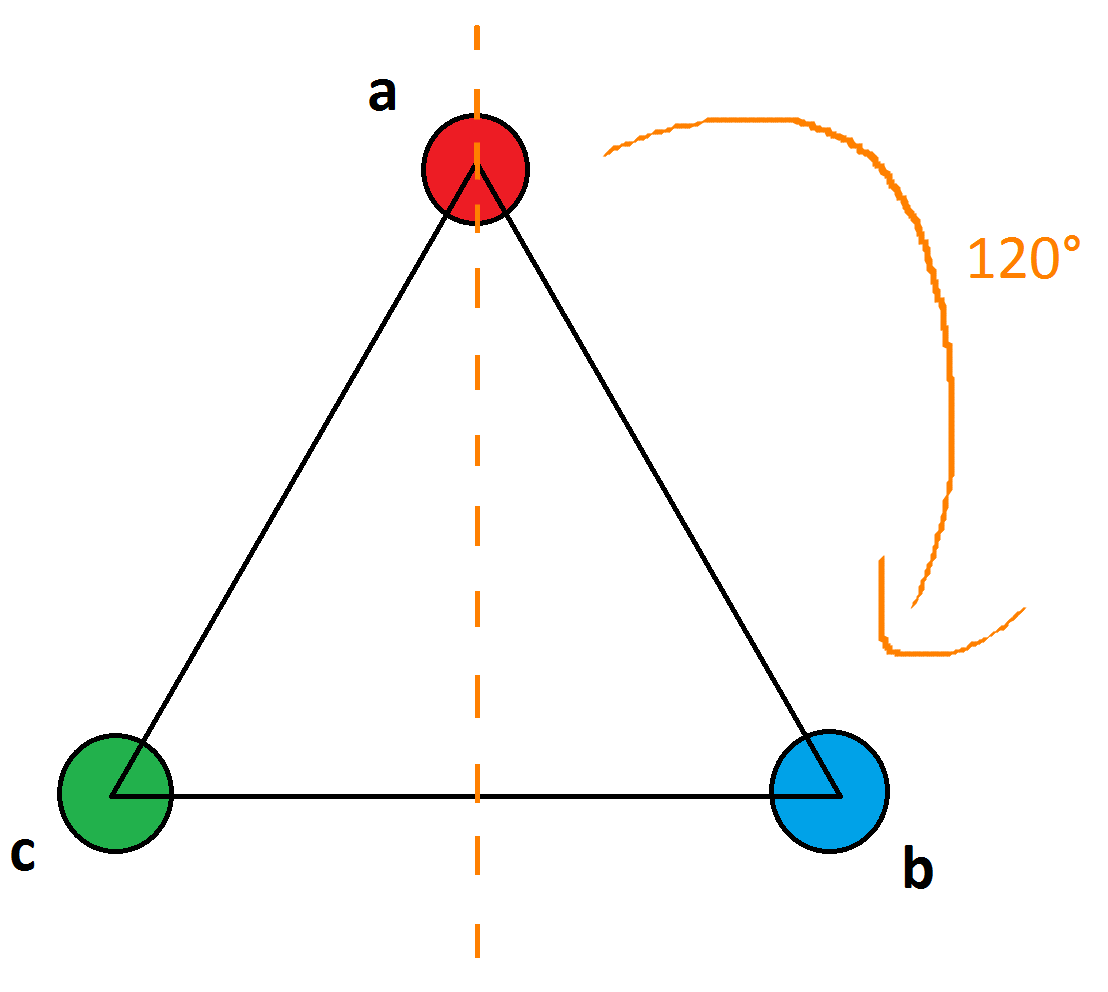
\includegraphics[width=1\linewidth]{src/GleichseitigUndGeschmeidig.png}
		%permutation of the vertexes, that maps edges on same positions
		%identiy, reflection on the perpendicular between b and c, 120 degree rotation clockwise
	\end{columns}
}
\frame[t]{
	\frametitle{From genes to nervous systems}
	\begin{itemize}
		\item Evolutionary algorithms for generation of ANNs
		%as it is happening in nature
		%An encoding of the network structure as genotype has to be defined
		\item An encoding of the network structure as genotype has to be defined
		\item Developmental encodings
		\begin{itemize}
			\item Definition of abstract constructions rules
			%like defining the properties of a whole field of neurons
		\end{itemize}
		\item Direct encodings
		\begin{itemize}
			\item Direct mapping of genotype to phenotype
			%describing each neuron individually
		\end{itemize}
		%during this short presentation I don't explain the different encodings further
	\end{itemize}
}
\frame[t]{
	\frametitle{Skinner box}
	\begin{columns}
		\column{1\textwidth}
		\begin{itemize}
			\item Experimental setup to test the learning ability of a test subject
			%stimulators
		\end{itemize}
		%\column{.4\textwidth}
		%\hspace*{-0.2cm}
		%\centering
		%\includegraphics[width=0.4\linewidth]{src/Skinner_box_scheme_01.png}
		\vspace*{-1cm}
		\begin{figure}[h]
			\begin{center}
				\includegraphics[width=.4\textwidth]{Skinner_box_scheme_01.png}
			\end{center}
			\vspace*{-0.2cm}
			\caption*{{\tiny \url{https://commons.wikimedia.org/wiki/File:Skinner_box_scheme_01.png}}}
		\end{figure}
		
		%test animal is supposed to associate some input stimuli to the appropriate action response
		%food and electric shocks used to support/punish right/wrong behaviour
	\end{columns}
}
\section{Approach}
\frame[t]{
	\frametitle{Experimental setup}
	\begin{itemize}
		\item ANNs are trained and tested in the environment of a simulated Skinner box
	\end{itemize}
	%\centering
	%\includegraphics[width=0.45\linewidth]{src/network_structure.png}
	%\vspace*{-1cm}
	\begin{columns}
		\column{.65\textwidth}
		\begin{itemize}
			\item An association set is a set that relates each input to an output e.g. {\small $\left\{(1,C),(2,D),(3,B),(4,A)\right\}$}
			\item The evolutionary algorithm uses a subset of all possible association sets (training set) %for the evaluation of its fitness function
		\end{itemize}
		\column{.4\textwidth}
		\begin{figure}[h]
			\begin{center}
				\includegraphics[width=1\textwidth]{network_structure.png}
			\end{center}
			%\vspace*{-0.2cm}
			\caption*{\textsuperscript{[Tonelli and Mouret, 2013]}}
		\end{figure}
	\end{columns}
}
\frame[t]{
	\frametitle{A step in the evaluation of an ANN}
	%modulatory neurons use the reward signals
	%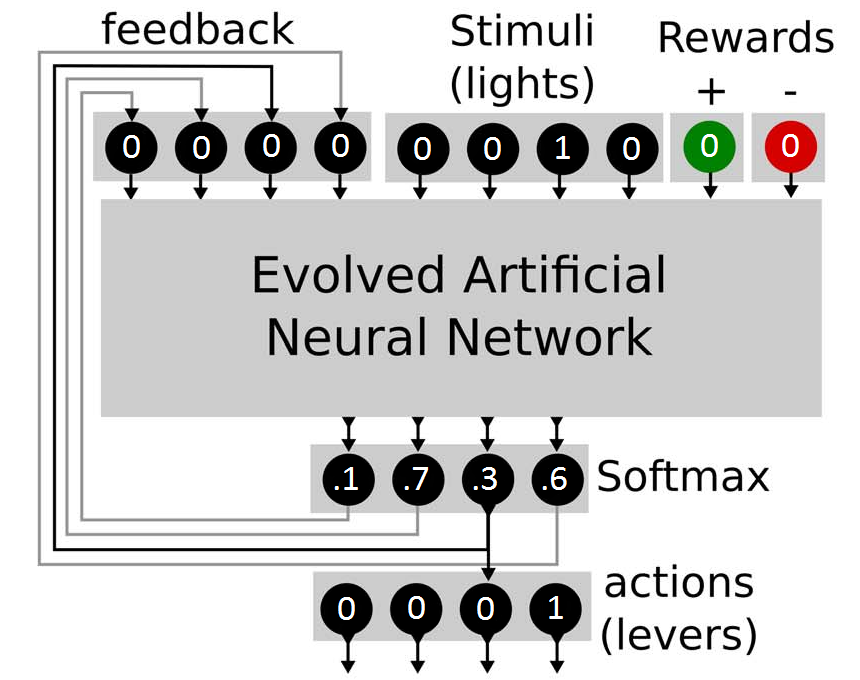
\includegraphics[width=0.45\linewidth]{src/network_structure_input1.png}
	\begin{figure}
		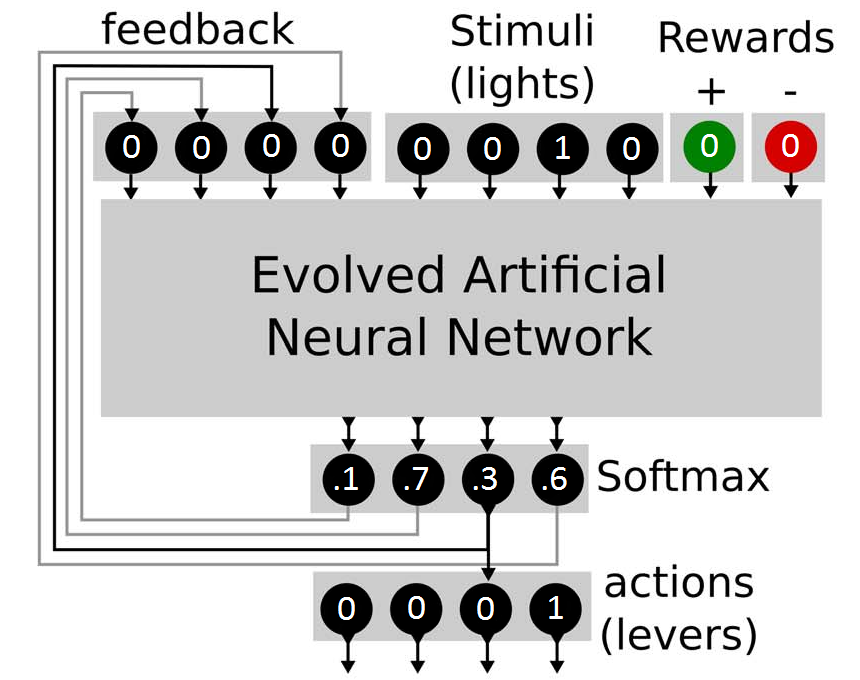
\includegraphics[width=.4\textwidth]{src/network_structure_input1.png}
		%\vspace*{-0.2cm}		
		\hfill
		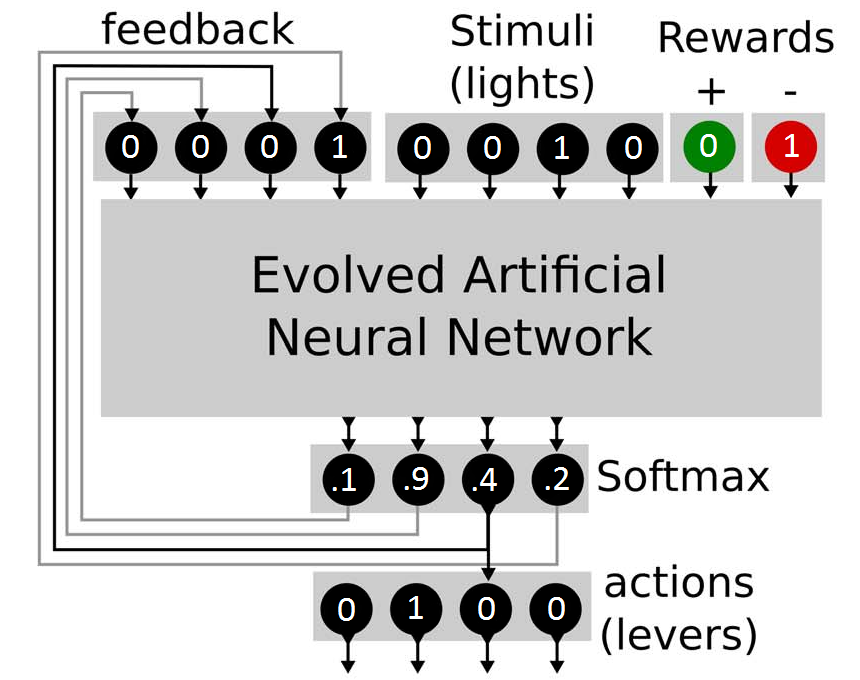
\includegraphics[width=0.4\linewidth]{src/network_structure_input2.png}
		%\caption*{Based on \textsuperscript{[Tonelli and Mouret, 2013]}}
		\caption*{{\tiny Based on [Tonelli and Mouret, 2013]}}
	\end{figure}
	\begin{itemize}
		\item Weights in the network are changed with modulatory neurons
		% should associate stimuli to actions by working with the signals
		%no direct influence on the ANN, it has to 
		%enables the ANN to learn something by changing connection weights
	\end{itemize}
}
\frame[t]{
	\frametitle{A run of the experiment}
	\begin{itemize}
		\item Choose a genetic encoding (direct or developmental)
		\item Select an evolutionary training set
		\item Develop ANNs that perform well on the training set
		\item Calculate the general learning ability (GLA) of the ANNs by evaluating their performance on unseen association sets
		%count the number of correct learned associations
		\item Evaluate the regularity by counting the graph automorphisms
	\end{itemize}
}

\section{Results}
\frame[t]{
	\frametitle{Results}
	%\vspace*{-0.8cm}
	\begin{itemize}
		\item All \textit{solutions} hold at least one modulatory neuron
		%solutions are ANNs with perfect score on the evolutionary training set
		%plasticity can only be achieved with modulatory neurons  
	\end{itemize}
	%\hspace*{-0.47cm}
	%\includegraphics<2>[width=1.072\linewidth]{src/results.png}
}
\frame[t]{
	\frametitle{Results}
	\vspace*{-1.15cm}
	\begin{figure}
		\hspace*{-0.515cm}
			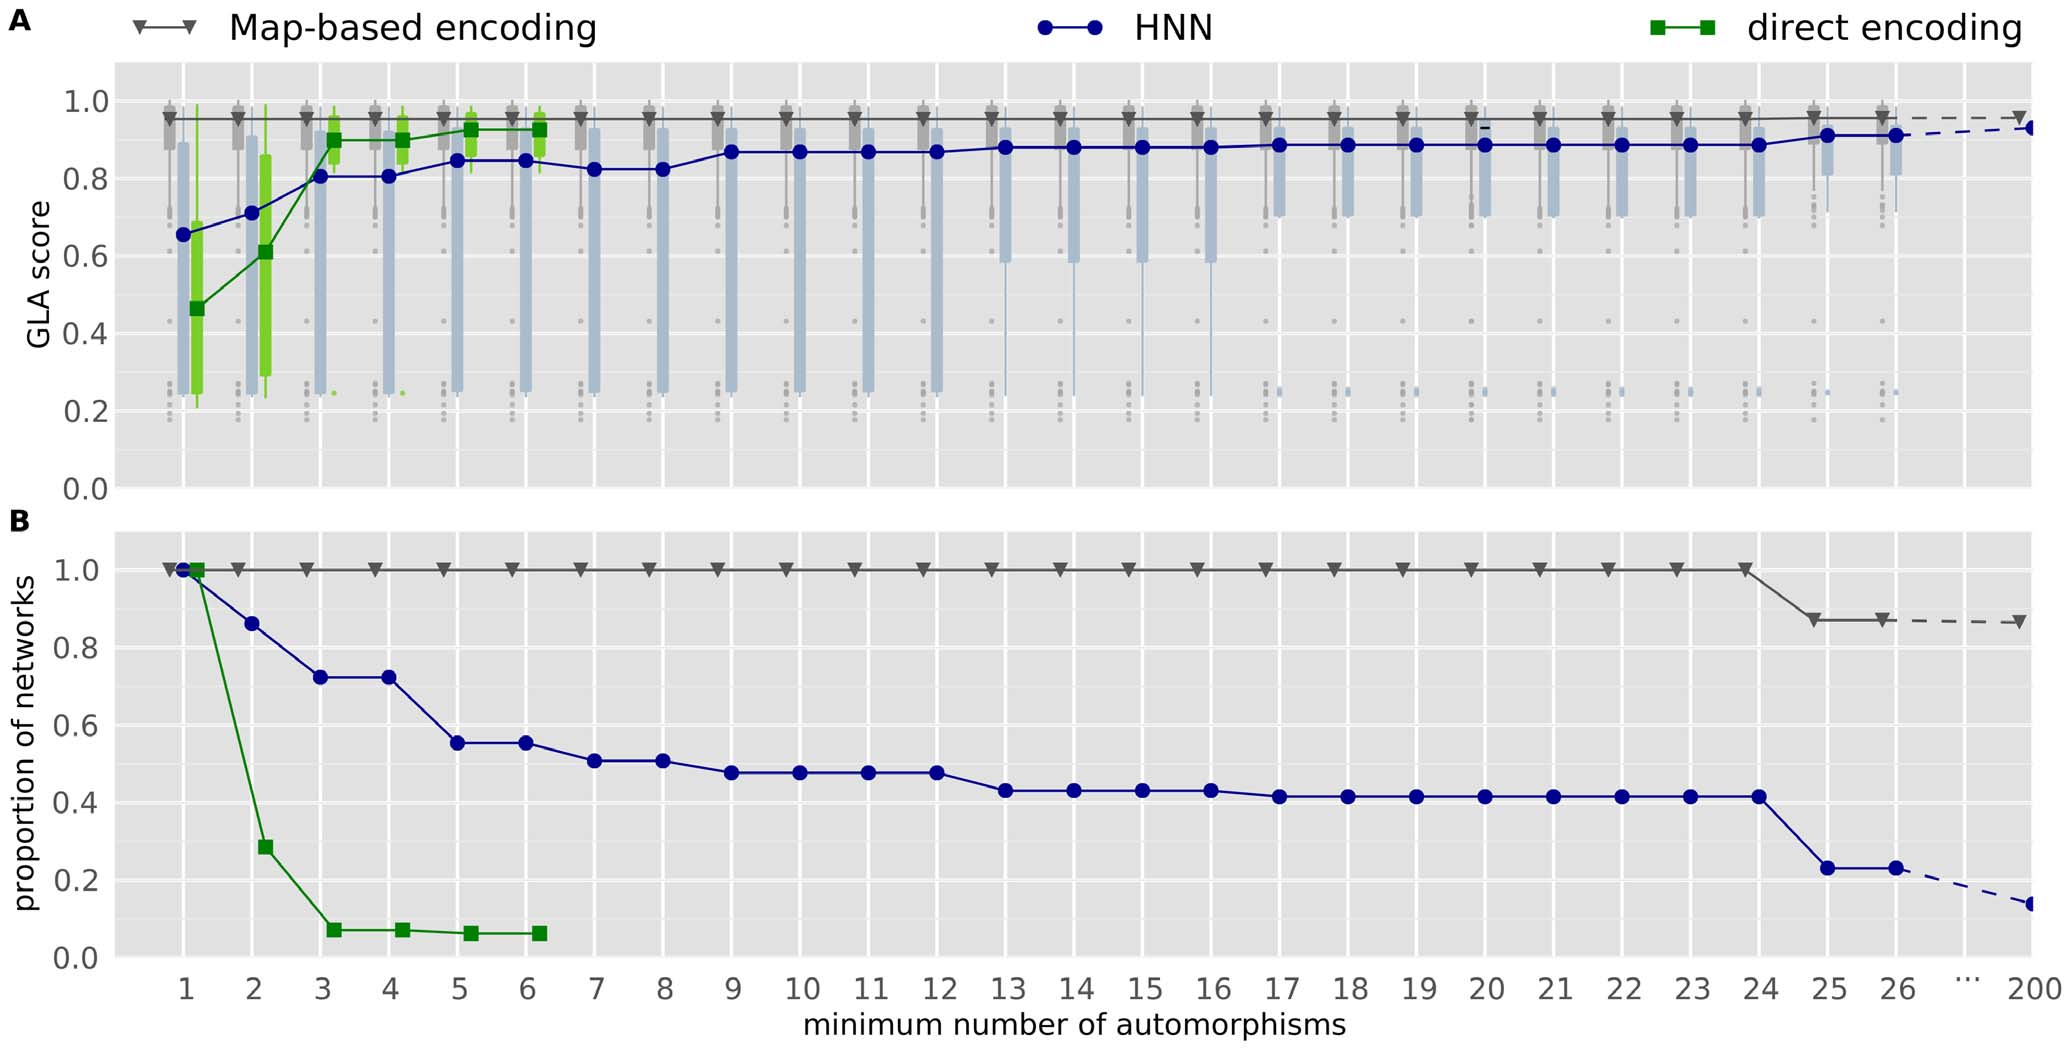
\includegraphics[width=1.077\textwidth]{src/results.png}
		%\vspace*{-0.2cm}
		\caption*{\textsuperscript{[Tonelli and Mouret, 2013]}}
	\end{figure}
		%A: number of graph automorphisms positively correlated to its GLA score
		%B: developmental encodings produce more graph automorphisms thatn direct enc		
}
\section{Conclusion}
\frame[t]
{
  \frametitle{Conclusion}

%ANNs general learning ability for different genetic encodings got tested
  \begin{itemize}
	  \item Plasticity and genetic encoding should be studied together
	    \begin{itemize}
	    	\item Developmental encodings lead to more more regular network structures than direct encodings
	    	\item Higher regularity leads to better general learning ability
	    \end{itemize}
		%\item The genetic encoding is an important aspect for the development of animal like nervous systems 
  \end{itemize}

\mbox{ }
  
	Open Question:
  \begin{itemize}
  	%\item Do few graph automorphisms imply low regularity?
  	%small changes lead to no graph automorphisms
  	\item Do plasticity and trainability have a trade-off relationship?
  	%the advantage in flexibility is achieved through redundante network parts
  	%a more complex task for the ANNs might impair the advantages of regular networks, because they are bigger and therefore harder to train
  \end{itemize}
}

%%%%%%%%%%%%%%

\frame[c]{
  \frametitle{The End}
\begin{center}
  Thank you for your attention.\\[1ex]
  Any question?\\[5ex]
\end{center}
  \footnotesize
  Literature:
	\begin{itemize}
		\item Paul Tonelli and Mouret Jean-Baptiste. On the Relationships between Generative Encodings, Regularity, and Learning Abilities when Evolving Plastic Artificial Neural Networks. \emph{PLoS ONE}, 2013
	
		%\item Paul Tonelli and Mouret Jean-Baptiste. Name of the conference paper. \emph{In: Proceedings of the Conference Name}, 2008
		%\item Author, Author, and Author. Name of the Article. \emph{Name of the Journal}, 42:111-133, 2010
		%\item Author, and Author. \emph{Name of the Book}. Publisher, 2009
	\end{itemize}
}

\end{document}
